\documentclass[12pt, a4paper,titlepage]{report}
\usepackage[utf8]{inputenc}
\usepackage[english]{babel}

%\usepackage{algorithm,algorithmic}

\usepackage{hyperref}
\hypersetup{
	linktoc=all
}

% Math symbols and utility
\usepackage{mathtools}
\usepackage{amsmath}
\usepackage{amssymb}
\usepackage{bm}

% Graphics
\usepackage{graphicx}
\graphicspath{ {images/} }
\usepackage{tikz}

\usepackage{fancyhdr}
\pagestyle{fancy}
\fancyhead{}
\fancyhead[RO,LE]{EdgeLearning}
\fancyfoot{}
\fancyfoot[LE,RO]{\thepage}
\fancyfoot[LO,CE]{Chapter \thechapter}
\fancyfoot[CO,RE]{Mirco De Marchi}

%\usepackage{xcolor}
%\definecolor{deepblue}{rgb}{0,0,0.5}
%\definecolor{deepred}{rgb}{0.6,0,0}
%\definecolor{deepgreen}{rgb}{0,0.5,0}
%\definecolor{maroon}{rgb}{0.5,0,0}

\usepackage{listings}

% Table environment
\usepackage{array, longtable}
\usepackage{tabularx}
\renewcommand{\arraystretch}{1.2}

% Force table position
\usepackage{float}
\restylefloat{table}

\begin{document}
	\begin{titlepage}
		\begin{center}
			\vspace*{2cm}
			
			\normalsize
			Project Documentation
			
			\vspace{2.5cm}
			
			\Huge
			\textbf{EdgeLearning}
			\vspace{0.5cm}
			
			\large
			Deep Learning for EdgeLearning
			
			\vspace{3cm}
			
			\large
			\textbf{Mirco De Marchi}
			
			\vspace{5cm}
		\end{center}
	\end{titlepage}
	
	\tableofcontents
	
	% INTRODUCTION
	\chapter{Introduction}
	EdgeLearning is a tool for reachability analysis and model checking of hybrid systems. Additionally, EdgeLearning is a framework for rigorous computation featuring arithmetic, linear algebra, calculus, geometry, algebraic and differential equations, and optimization solvers.

EdgeLearning wants to be a library that extends EdgeLearning functionalities in order to provide online estimations of the running system to improve its execution through Machine Learning and Deep Learning techniques. In particular, EdgeLearning focuses on 2 main use case: 
\begin{itemize}
	\item Task execution time estimation;
	\item Adaptation of the dynamic part of a hybrid system model;
\end{itemize}

The implementation has to be done in C++ and it can be based on a library for Machine Learning and Deep Learning, with strict compatibility for the major operating systems. As alternative, the library can be developed from zero, in order to build an ad-hoc implementation. The library has to be compatible with MacOS, Ubuntu, Debian and Windows, in particular the library has to be provided by the following package manager: \href{https://brew.sh}{Homebrew}, \href{https://wiki.debian.org/Aptitude}{Aptitude} and \href{https://docs.microsoft.com/it-it/cpp/build/vcpkg?view=msvc-160}{vcpkg}. The libraries discussed will be the following: 
\begin{itemize}
	\item Tensorflow: \href{https://github.com/tensorflow/tensorflow}{github.com/tensorflow}, \href{https://www.tensorflow.org}{/www.tensorflow.org};
	\item Caffe: \href{https://github.com/BVLC/caffe}{github.com/caffe}, \href{http://caffe.berkeleyvision.org}{caffe.org};
	\item Cognitive Toolkit (CNTK): \href{https://github.com/microsoft/CNTK}{github.com/CNTK}, \href{https://docs.microsoft.com/it-it/cognitive-toolkit/}{docs.microsoft.com/cognitive-toolkit};
	\item dynet: \href{https://github.com/clab/dynet}{github.com/dynet}, \href{http://dynet.io}{dynet.io};
	\item shogun: \href{https://github.com/shogun-toolbox/shogun}{github.com/shogun}, \href{https://www.shogun.ml}{www.shogun.ml};
	\item FANN: \href{https://github.com/libfann/fann}{github.com/fann}, \href{http://leenissen.dk/fann/wp/}{leenissen.dk/fann};
	\item Shark library: \href{https://github.com/Shark-ML/Shark}{github.com/Shark}, \href{http://www.shark-ml.org}{www.shark-ml.org};
	\item OpenNN: \href{https://github.com/Artelnics/OpenNN}{github.com/OpenNN}, \href{https://www.opennn.net}{www.opennn.net};
	\item mlpack: \href{https://github.com/mlpack/mlpack}{github.com/mlpack}, \href{https://www.mlpack.org}{www.mlpack.org};
	\item Boost: \href{https://github.com/boostorg/boost}{github.com/boost}, \href{https://www.boost.org}{www.boost.org};
	\item Eigen3: \href{https://gitlab.com/libeigen/eigen}{gitlab.com/eigen}, \href{https://eigen.tuxfamily.org/index.php?title=Main_Page}{eigen.tuxfamily.org};
	\item Armadillo: \href{https://gitlab.com/conradsnicta/armadillo-code}{gitlab.com/armadillo}, \href{http://arma.sourceforge.net}{arma.sourceforge.net}
\end{itemize}


The following list provides some useful links related to the implementation and other resources: 
\begin{itemize}
	\item EdgeLearning main repository: \href{https://github.com/ariadne-cps/ariadne}{github.com/ariadne-cps/ariadne};
	\item EdgeLearning extension repository: \href{https://github.com/mircodemarchi/EdgeLearning}{github.com/mircodemarchi/EdgeLearning};
\end{itemize}
	
	% REQUIREMENTS
	\chapter{Requirements}
	\section{Task execution time estimation}

The first EdgeLearning integration is the \textbf{estimation of task execution time}. EdgeLearning can execute in parallel multiple tasks, that are represented as numeric integrations of a set that evolves over time. The tasks amount executed during the system evolution before the global integration finishes, is quite a large number. The objective is to find the best schedule of the task with different configurations, in order to obtain the best result in terms of execution time. This implementation can be useful in EdgeLearning, because different tasks could have really different execution time and the predicted execution time of a specified task configuration can be used to improve the threads scheduling. 

Let assume to take in input a vector of bounded integer values, that represents the task parameters configuration for the numeric integration, the output has to be the estimated execution time of input task in microseconds. The task takes another input, in addition to the numeric configuration, that is the initial state of the set. The set is represented as a Taylor expansion with dozen of terms related with the continuous variables of the set space, that is more difficult to represent in the training model of a neural network. The set state has to be taken in consideration during the evolution of system tasks, because the task execution time tends to vary during the temporal evolution of the set, according to its complexity. 

The deep learning model can be initially trained with a sequence of task parameters configurations labelled with their execution time. Then the estimator model has to take in input a task configuration and produce the predicted execution time. Even if the system has to perform multiple task in concurrence, the estimator model is interested in each single task execution. For this reason the most suitable solution for this integration would be a simple Feedforward Neural Network (FNN), without too many layers, in order to avoid an excessive storage of training data.

The prediction model can be improved over time, because when tasks finish their execution, EdgeLearning keeps track of real execution time. Furthermore, the deep learning model has to work well for the last evolution time interval rather than for all evolution, therefore it has to loose memory of oldest executions during online learning and overfitting has to be avoided. To implement this, the estimator has to provide an online learning, in order to give more importance to the latest execution time results obtained.


\section{Parametric dynamic system adaptation}

The second EdgeLearning integration is the \textbf{adaptation of a parametric function that represents the dynamic part of a hybrid system model}. Given a vector of samples, defined on continuous variables, that represent the states of a real system, and an associated hybrid model, we want to get the best accuracy of the hybrid model compared to the real system. Since time evolution is faster than real system evolution, we can use the hybrid model to predict in advance the points that the real system will reach, in order to catch dangerous situations. However, if the hybrid model is not so accurate, the performed prediction will be inaccurate. 

The accuracy of this hybrid model can be improved through some configurable parameters that are given to the functions associated with the model dynamic at each location. The parameters can be defined as point values or, more generally, intervals, and allow to include the samples evolution. In fact, the hybrid model evolution can be represented as a flow channel that is the time evolution of a non-punctual set. The narrower the flow channel, the more accurate the model prediction and the greater the likelihood of including samples of real evolution in the flow channel defined by the sequence of chosen parameters.

The hybrid model evolution is periodically repeated starting from the last sample received by the real system. Therefore, the hybrid model can learn how to improve the sequence of chosen parameter through its errors. The proposed solution is to integrate a deep learning model inside the hybrid model that periodically takes as input the real system state, defined as a sequence of continuous variable samples, and it has to give as output the parameters values for the parametric functions of each dynamic model location that allow the hybrid model to best return a set of points that includes the future real system samples. The output has to be given as an interval, that is a minimum-maximum pair. 

The deep learning model can be trained with a sequence of samples produced by the real system and a related sequence of simulated values produced by the hybrid model of the real system, with a defined parametric function for each hybrid model locations. In addition, the estimator has to be able to improve periodically the accuracy during system execution, for this reason the model has to perform an online learning. Ideally, in a real system that perform over a loop, the learning phase should be executed along all the samples collected in the loop. However, since the loop period is not easily findable, the number of samples on which perform the learning phase is not defined. Finally, this solution needs to define a quality metric of the estimator.

Furthermore, the prediction could be improved with an inference performed along a sequence of samples, because a future state can be found more accurately if the learning model had some of the past sequence of states available. For example a past sequence of states might suggest a direction of the states evolution, if the states evolution is located around a limited area or if it spreads over a large area. For this reason the most suitable solution would be a Recurrent Neural Network (RNN), because it suits really well with temporal sequences. However, the RNN learning model works very well if the real system future state depends on a sequence of previous states, but if the evolution states of a real system depends only on the current state, the usefulness of RNN decreases.

Since there is not a strict necessity to avoid overfitting and the complexity of this use case, compared to the first one, is higher, a good solution could be to implement a Feedforward Neural Network (FNN) with a larger amount of layers, in order to manage better a difficult problem. Therefore, if the RNN does not provide good results then you could opt for the FNN solution.

	
	% DEEP LEARNING C++ LIBRARY ANALISYS
	\chapter{C++ Libraries}
	\input{chapters/chapter03deeplearning-lib-analysis}
	
	% IMPLEMENTATION
	\chapter{Implementation}
	\section{FNN: Forward Neural Network}

\subsection{Background}\label{background}

Suppose we have a task we would like a machine learning model to
complete (e.g.~recognizing handwritten digits). At a high level, we need
to perform the following tasks:

\begin{enumerate}
	\item
	First, we must conceptualize the task as a ``function'' such that the
	inputs and outputs of the task can be described in a concrete
	mathematical sense (amenable for programmability).
	\item
	Second, we need a way to quantify the degree to which our model is
	performing poorly against a known set of correct answers. This is
	typically denoted as the \emph{loss} or \emph{objective} function of
	the model.
	\item
	Third, we need an \emph{optimization strategy} which will describe how
	to adjust the model after feedback is provided regarding the model's
	performance as per the loss function described above.
	\item
	Fourth, we need a \emph{regularization strategy} to address
	inadvertently tuning the model with a high degree of specificity to
	our training data, at the cost of generalized performance when
	handling inputs not yet encountered.
	\item
	Fifth, we need an \emph{architecture} for our model, including how
	inputs are transformed into outputs and an enumaration of all the
	adjustable parameters the model supports.
	\item
	Finally, we need a robust \emph{implementation} that executes the
	above within memory and execution budgets, accounting for
	floating-point stability, reproducibility, and a number of other
	engineering-related matters.
\end{enumerate}

\emph{Deep learning} is distinct from other machine learning models in
that the architecture is heavily over-parameterized and based on simpler
\emph{building blocks} as opposed to bespoke components. The building
blocks used are neurons, or particular arrangements of neurons,
typically organized as layers. Over the course of training a deep
learning model, it is expected that \emph{features} of the inputs are
learned and manifested as various parameter values in these neurons.
This is in contrast to traditional machine learning, where features are
not learned, but implemented directly.

\subsection{Categorical Cross-EntropyLoss}\label{categorical-cross-entropy-loss}

More concretely, the task at hand is to train a model to recognize a 28
by 28 pixel handwritten greyscale digit. For simplicity, our model will
interpret the data as a flattened 784-dimensional vector. Instead of
describing the architecture of the model first, we'll start with
understanding what the model should output and how to assess the model's
performance. The output of our model will be a 10-dimensional vector,
representing the probability distribution of the supplied input. That
is, each element of the output vector indicates the model's estimation
of the probability that the digit's value matches the corresponding
element index. For example, if the model outputs:

\[M(\mathbf{I}) = \left[0, 0, 0.5, 0.5, 0, 0, 0, 0, 0, 0\right]\]

for some input image \(\mathbf{I}\), we interpret this to mean that the
model believes there is an equal chance of the examined digit to be a 2
or a 3.

Next, we should consider how to quantify the model's loss. Suppose, for
example, that the image \(\mathbf{I}\) actually corresponded to the
digit ``7'' (our model made a horrible prediction!), how might we
penalize the model? In this case, we know that the \emph{actual}
probability distribution is the following:

\[\left[0, 0, 0, 0, 0, 0, 0, 1, 0, 0\right]\]

This is known as a ``one-hot'' encoded vector, but it may be helpful to
think of it as a probability distribution given a set of events that are
mutually exclusive (a digit cannot be both a ``7'' \emph{and} a ``3''
for instance).

Fortunately, information theory provides us some guidance on defining an
easy-to-compute loss function which quantifies the dissimilarities
between two probability distributions. If the probability of of an event
\(E\) is given as \(P(E)\), then the \emph{entropy} of this event is
given as \(-\log P(E)\). The negation ensures that this is a positive
quantity, and by inspection, the entropy increases as an event becomes
less likely. Conversely, in the limit as \(P(E)\) approaches \(1\), the
entropy shrinks to \(0\). While several interpretations of entropy are
possible, the pertinent interpretation here is that entropy is a
\emph{measure of the information conveyed when a particular event
	occurs}. That the ``sun rose this morning'' is a fairly mundane
observation but being told ``the sun exploded'' is sure to pique your
attention. Because we are reasonably certain that the sun rises each
morning (with near 100\% confidence), that ``the sun rises'' is an event
that conveys little additional information when it occurs.

Let's consider next entropy in the context of a probability
distribution. Given a discrete random variable \(X\) which can take on
values \(x_0, \dots, x_{n-1}\) with probabilities
\(p(x_0), \dots, p(x_{n-1})\), the entropy of the random variable \(X\)
is defined as:

\[H(X) = -\sum_{x \in X} p(x) \log p(x)\]

For example, suppose \(W\) is a binary random variable that represents
today's weather which can either be ``sunny'' or ``rainy'' (a binary
random variable). The entropy \(H(W)\) can be given as:

\[H(W) = -S\log S - (1 - S) \log (1 - S)\]

where \(S\) is the probability of a sunny day, and hence \(1 - S\) is
the probability of a rainy day. As a binary random variable, the
summation over weighted entropies expands to only two terms. What does
this quantity mean? If we were to describe it in words, each term of the
sum in the entropy calculation corresponds to the information of a
particular event, weighted by the probability of the event. Thus, the
entropy of the distribution is literally the \emph{expected amount of
	information contained in an event} for a given distribution. If we plot
\(-S\log S - (1 - S) \log(1 - S)\) as a function of \(S\), we will see
something like this:

\begin{figure}
	\centering
	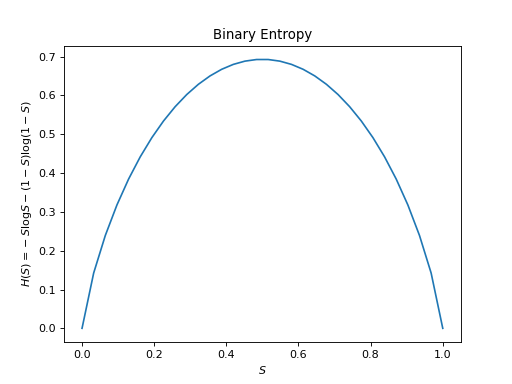
\includegraphics{cross_entropy.png}
	\caption{Cross Entropy matching distribution}
	\label{fig:cross_entropy} 
\end{figure}

As a minor note, while \(\log 0\) is an undefined quantity, information
theorists accept that \(\lim_{p\rightarrow 0} p\log p = 0\) by
convention. Intuitively, the expected entropy should be unaffected by
the set of impossible events.

As you might expect, when the distribution is 50-50, the uncertainty of
a binary is maximal, and by extension the amount of information
contained in each event is maximized too. Put another way, if you lived
in an area where it was always sunny, you wouldn't \emph{learn anything}
if someone told you it was sunny today. However, in a tropical region
characterized by capricious weather, information conveyed about the
weather is far more meaningful.

In the previous example, we weighted the event entropies according to
the event's probability distribution. What would happen if, instead, we
used weights corresponding to a \emph{different} probability
distribution? This is known as the \emph{cross entropy}:

\[H(p, q) = -\sum_{x \in X} p(x)\log q(x)\]

To get some intuition about this, first, we note that if
\(p(x) = q(x), \forall x\in X\), the cross entropy trivially matches the
self-entropy. Let's go back to our binary entropy example and visualize
what it looks like if we chose a completely \emph{incorrect}
distribution. Specifically, suppose we computed the cross entropy where
if the probability of a sunny day is \(S\), we weight the entropy with
\(1 - S\) instead of \(S\) as in the self-entropy formula.

\begin{figure}
	\centering
	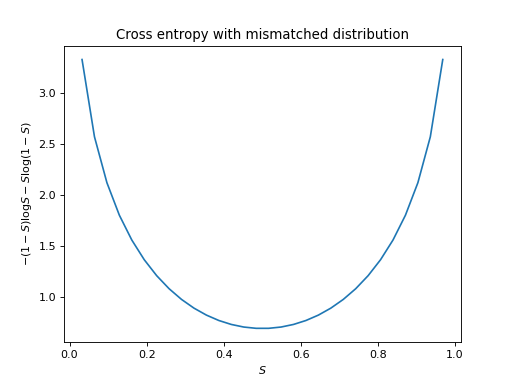
\includegraphics{cross_entropy_mismatch.png}
	\caption{Cross Entropy mismatching distribution}
	\label{fig:cross_entropy_mismatch}
\end{figure}

If you compare the values with the previous figure, you'll see that the
cross entropy diverges from the self-entropy everywhere except \(0.5\),
where \(S = 1 - S\). The difference between the cross entropy
\(H(p, q)\) and entropy \(H(p)\) provides then, a \emph{measure of
	error} between the presumed distribution \(q\) and the true distribution
\(p\). This difference is also known as the
\href{https://en.wikipedia.org/wiki/Kullback\%E2\%80\%93Leibler_divergence}{Kullback-Leibler
	divergence} or KL divergence for short.

Given that the entropy of a given probability distribution \(p\) is
constant, then \(H(p)\) must be constant as well. This is why in
practice, we will generally seek to minimize the cross entropy between
\(p\) and a predicted distribution \(q\), which by extension will
minimize the Kullback-Leibler divergence as well.

Now, we have the tools to know if our model is succeeding or not! Given
an estimation of a sample's label as before:

\[M(\mathbf{I}) = \left[0, 0, 0.5, 0.5, 0, 0, 0, 0, 0, 0\right]\]

we will treat our model's output as a predicted probability distribution
of the sample digit's classification from 0 to 9. Then, we compute the
cross entropy between this predction and the true distribution, which
will be in the form of a one-hot vector. Supposing the actual digit is 3
in this particular case (\(P(7) = 1\)):

\[ \sum_{x\in \{0,\dots, 9\}} -P(x) \log Q(x) = -P(3) \log(Q(3)) = \log(0.5) \approx 0.301 \]

Let's make a few observations before continuing. First, for a one-hot
vector, the entropy is 0 (can you see why?). Second, by pretending the
correct digit above is \(3\) and not, say, \(7\), we conveniently
avoided \(\log 0\) showing up in the final expression. A common method
to avoid this is to add a small \(\epsilon\) to the log argument to
avoid this singularity, but we'll discuss this in more detail later.

\subsection{Approximation Function with a Neural
		Network}\label{approximation-function-with-a-neural-network}

Now that we know how to evaluate our model, we'll need to decide how to
go about making predictions in the form of a probability distribution.
Our model will need to take as inputs, 28x28 images (which as mentioned
before, will be flattened to 784x1 vectors for simplicity). Let's
enumerate the properties our model will need:

\begin{enumerate}
	\item
	Parameterization - our model will need parameters we can adjust to
	``fit'' the model to the data
	\item
	Nonlinearity - it is assuredly not the case that the probability
	distribution can be modeled with a set of linear equations
	\item
	Differentiability - the gradient of our model's output with respect to
	any given parameter indicates the \emph{impact} of that parameter on
	the final result
\end{enumerate}

There are an infinite number of functions that fit this criteria, but
here, we'll use a simple feedforward network with a single hidden layer.

\begin{center}
	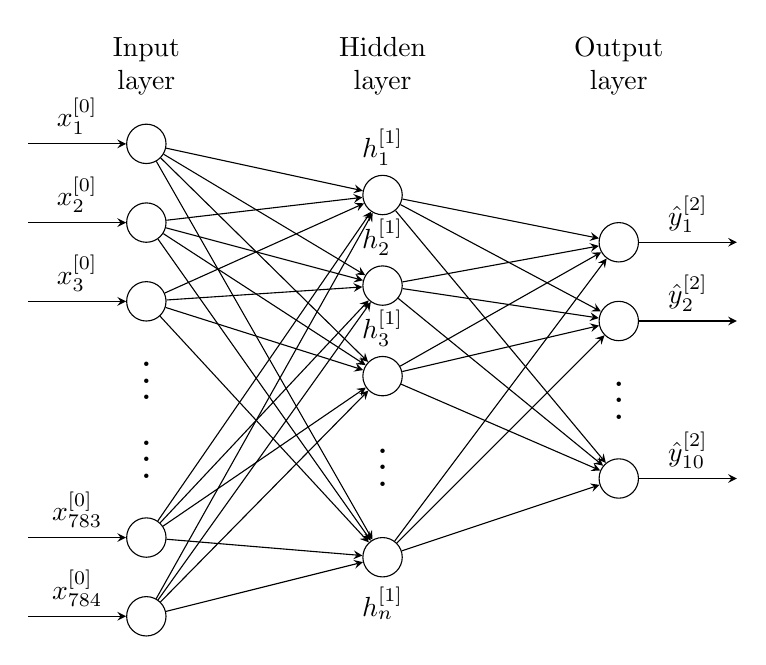
\begin{tikzpicture}[x=1.5cm, y=1cm, >=stealth]
		
		\tikzset{%
			every neuron/.style = {
				circle,
				draw,
				minimum size=0.5cm
			},
			neuron missing/.style = {
				draw=none,
				scale=1.5,
				text height=0.3333cm,
				execute at begin node=\color{black}$\vdots$
			}
		}
		
		
		\foreach \m/\l [count=\y] in {1,2,3,missing,missing,783,784}
		\node [every neuron/.try, neuron \m/.try] (input-\m) at (0,2.5-\y) {};
		
		\foreach \m [count=\y] in {1,2,3,missing,4}
		\node [every neuron/.try, neuron \m/.try ] (hidden-\m) at (2,2-\y*1.15) {};
		
		\foreach \m [count=\y] in {1,2,missing,10}
		\node [every neuron/.try, neuron \m/.try ] (output-\m) at (4,1.25-\y) {};
		
		\foreach \l in {1,2,3,783,784}
		\draw [<-] (input-\l) -- ++(-1,0)
		node [above, midway] {$x_{\l}^{[0]}$};
		
		\foreach \l [count=\i] in {1,2,3}
		\node [above] at (hidden-\i.north) {$h_\l^{[1]}$};
		
		\node [below] at (hidden-4.south) {$h_n^{[1]}$};
		
		\foreach \l in {1,2,10}
		\draw [->] (output-\l) -- ++(1,0)
		node [above, midway] {$\hat{y}_{\l}^{[2]}$};
		
		\foreach \i in {1,2,3,783,784}
		{
			\draw [->] (input-\i) -- (hidden-4);
			\foreach \j in {1,...,3}
			\draw [->] (input-\i) -- (hidden-\j);
		}
		
		\foreach \i in {1,2,3,4}
		{
			\draw [->] (hidden-\i) -- (output-10);
			\foreach \j in {1,...,2}
			\draw [->] (hidden-\i) -- (output-\j);
		}
		
		\foreach \l [count=\x from 0] in {Input, Hidden, Output}
		\node [align=center, above] at (\x*2,2) {\l \\ layer};
		
	\end{tikzpicture}
\end{center}

A few quick notes regarding notation: a superscript of the form \([i]\)
is used to denote the \(i\)th layer. A subscript is used to denote a
particular element within a layer or vector. The vector \(\mathbf{x}\)
is usually reserved for training samples, and the vector \(\mathbf{y}\)
is typically reserved for sample labels (i.e.~the desired ``answer'' for
a given sample). The vector \(\hat{\mathbf{y}}\) is used to denote a
model's predicted labels for a given input.

On the far left, we have the input layer with \(784\) nodes
corresponding to each of the 28 by 28 pixels in an individual sample.
Each \(x_i^{(0)}\) is a floating point value between 0 and 1 inclusive.
Because the data is encoded with 8 bits of precision, there are 256
possible values for each input. Each of the 784 input values fan out to
each of the nodes in the hidden layer without modification.

In the center hidden layer, we have a variable number of nodes that each
receive all 784 inputs, perform some processing, and fan out the result
to the output nodes on the far right. That is, each node in the hidden
layer transforms a \(\mathbb{R}^{784}\) vector into a scalar output, so
as a whole, the \(n\) nodes collectively need to map
\(\mathbb{R}^\rightarrow \mathbb{R}^n\). The simplest way to do this is
with an \(n\times 784\) matrix (treating inputs as column vectors).
Modeling the hidden layer this way, each of the \(n\) nodes in the
hidden layer is associated with a single row in our
\(\mathbb{R}^{n\times 784}\) matrix. Each entry of this matrix is
referred to as a \emph{weight}.

We still have two issues we need to address however. First, a matrix
provides a linear mapping between two spaces, and linear maps take \(0\)
to \(0\) (you can visualize such maps as planes through the origin).
Thus, such fully-connected layers typically add a \emph{bias} to each
output node to turn the map into an affine map. This enables the model
to respond zeroes in the input. Thus, the hidden layer as a whole has
now both a weight matrix, and also a bias vector. A linear mapping with
a constant bias is commonly referred to as an \emph{affine map}.

The second issue is that our hidden layer's now-affine mapping still
scales linearly with the input, and one of our requirements for our
approximation function was nonlinearity (a strict prerequisite for
universality). Thus, we perform one final non-linear operation the
result of the affine map. This is known as the \emph{activation
	function}, and an infinite number of choices present itself here. In
practice, the \emph{rectifier function}, defined below, is a perennial
choice.

\[f(x) = \max(0, x)\]

\begin{figure}
	\centering
	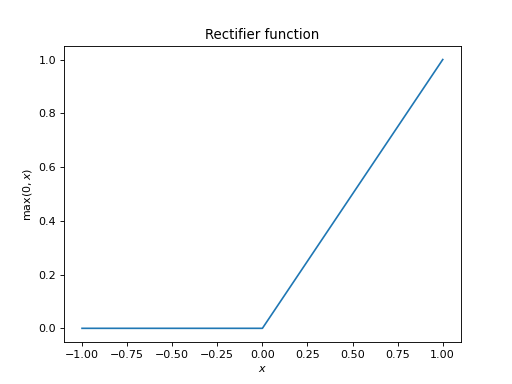
\includegraphics{relu.png}
	\caption{ReLU: Rectifier Linear Unit}
	\label{fig:relu}
\end{figure}

The rectifier is popular for having a number of desirable properties.

\begin{enumerate}

	\item
	Easy to compute
	\item
	Easy to differentiate (except at 0, which has not been found to be a
	problem in practice)
	\item
	Sparse activation, which aids in addressing model overfitting and
	``unlearning'' useful weights
\end{enumerate}

As our hidden layer units will use this rectifier just before emitting
its final output to the next layer, our hidden units may be called
\emph{rectified linear units} or ReLUs for short.

Summarizing our hidden layer, the output of each unit in the layer can
be written as:

\[a_i^{[1]} = \max(0, W_{i}^{[1]} \cdot \mathbf{x}^{[0]} + b_i^{[1]})\]

It's common to refer to the final activated output of a neural network
layer as the vector \(\mathbf{a}\), and the result of the internal
affine map \(\mathbf{z}\). Using this notation and considering the
output of the hidden layer as a whole as a vector quantity, we can
write:

\[
\begin{aligned}
	\mathbf{z}^{[1]} &= \mathbf{W}^{[1]}\mathbf{x}^{[0]} + \mathbf{b}^{[1]} \\
	\mathbf{a}^{[1]} &= \max(\mathbf{0}, \mathbf{z}^{[1]}) \\
	\mathbf{a}^{[1]}, \mathbf{b}^{[1]} &\in \mathbb{R}^n \\
	\mathbf{W}^{[1]} &\in \mathbb{R}^{n\times 784} \\
	\mathbf{x}^{[0]} &\in \mathbb{R}^{784}
\end{aligned}
\]

The last layer to consider is the output layer. As with the hidden
layer, we need a dimensionality transform, in this case, taking vectors
in \(\mathbb{R}^n\) and mapping them to vectors in \(\mathbb{R}^{10}\)
(corresponding to the 10 possible digits in the target output). As
before, we will use an affine map with the appropriately sized weight
matrix and bias vector. Here, however, the rectifier isn't suitable as
an activation function because we want to emit a probability
distribution. To be a valid probability distribution, each output of the
hidden layer must be in the range \([0, 1]\), and the sum of all outputs
must equal \(1\). The most common activation function used to achieve
this is the \emph{softmax function}:

\[\mathrm{softmax}(\mathbf{z})_i = \frac{\exp(z_i)}{\sum_j \exp(z_j)}\]

Given a vector input \(z\), each component of the softmax output (as a
vector quantity) is given as per the expression above. The exponential
functions conveniently map negative numbers to positive numbers, and the
denominator ensures that all outputs will be between 0 and 1, and sum to
1 as desired. There are other reasons why an exponential function is
used here, stemming from our choice of a loss function (based on the
underpinning notion of maximum-likelihood estimation), but we won't get
into that in too much detail here (consult the further reading section
at the end to learn more). Suffice it to say that an additional benefit
of the exponential function is its clean interaction with the logarithm
used in our choice of loss function, especially when we will need to
compute gradients in the next section.

Summarizing our neural network architecture, with two weight matrices
and two bias vectors, we can construct two affine maps which map vectors
in \(\mathbb{R}^{784}\) to \(\mathbb{R}^n\) to \(\mathbb{R}^{10}\).
Prior to forwarding the results of one affine map as the input of the
next, we employ an activation function to add non-linearity to the
model. First, we use a linear rectifier and second, we use a softmax
function, ensuring that we end up with a nice discrete probability
distribution with 10 possible events corresponding to the 10 digits.

Our network is small enough that we can actually write out the entire
process as a single function using the notation we've built so far:

\[f(\mathbf{x}^{[0]}) = \mathbf{y}^{[2]} = \mathrm{softmax}\left(\mathbf{W}^{[2]}\left(\max\left(\mathbf{0}, \mathbf{W}^{[1]}\mathbf{x}^{[0]} + \mathbf{b}^{[1]}\right) \right) + \mathbf{b}^{[1]} \right)\]

One thing to keep in mind here is that this implementation is \emph{not}
the most efficient implementation possible for a softmax layer feeding
to a cross-entropy loss function by any stretch. The code and derivation
here is completely general for arbitrary sample probability
distributions. If, however, we can assume that the target distribution
is one-hot encoded, then all gradients in this node will either be 0 or
\(-1/\hat{y}_k\) where \(k\) is the active label in the one-hot target.
Upon substitution in the previous layer, it should be clear that
important cancellations are possible that dramatically simplify the
gradient computations in the softmax layer. Here's the simplification,
again assuming that the \(k\)th index is the correct label:

\[
\begin{aligned}
	\frac{\partial J_{CE}}{\partial \mathrm{softmax}(\mathbf{z})_i} &= \frac{\partial J_{CE}}{\partial a_i}\sum_{j} \begin{cases}
		\mathrm{softmax}(\mathbf{z})_i\left(1 - \mathrm{softmax}(\mathbf{z})_i\right) & i = j \\
		-\mathrm{softmax}(\mathbf{z})_i \mathrm{softmax}(\mathbf{z})_j & i \neq j
	\end{cases} \\
	&= \begin{dcases}
		-\frac{\mathrm{softmax}(\mathbf{z})_k(1 - \mathrm{softmax}(\mathbf{z}_k))}{\mathrm{softmax}(\mathbf{z})_k} & i = k \\
		\frac{\mathrm{softmax}(\mathbf{z})_i\mathrm{softmax}(\mathbf{z})_k}{\mathrm{softmax}(\mathbf{z})_k} & i \neq k\\
	\end{dcases} \\
	&= \begin{dcases}
		\mathrm{softmax}(\mathbf{z})_k - 1 & i = k \\
		\mathrm{softmax}(\mathbf{z})_i & i \neq k
	\end{dcases}
\end{aligned}
\]

When following the computation above, remember that
\(\partial J_{CE} / \partial a_i\) is 0 for all \(i \neq k\). Thus, the
only term in the sum that survives is the term corresponding to
\(j = k\), at which point we break out the differentation depending on
whether \(i = k\) or \(i \neq k\).

This is an elegant result! Essentially, the gradient of a the loss with
respect to an emitted probability \(p(x)\) is simply \(p(x)\) if \(x\)
was not the correct label, and \(p(x) - 1\) if it was. Considering the
effect of gradient descent, this should check out with our intuition.
The optimizer seeks to suppress probabilities predicted that should have
been 0, and increase probabilities predicted that should have been 1.
Check for yourself that after gradient descent is performed, the
gradients derived here will nudge the model in the appropriate
direction.

This sort of optimization highlights an important observation about
backpropagation, namely, that backpropagation does not guarantee any
sort of optimality beyond a worst-case performance ceiling. Several
production neural networks have architectures that employ heuristics to
identify optimizations such as this one, but the problem of generating a
perfect computational strategy is NP and so not covered here. The code
provided here will remain in the general form, despite being slower in
the interest of maintaining generality and not adding complexity, but
you are encouraged to consider abstractions to permit this type of
optimization in your own architecture (a useful keyword to aid your
research is \emph{common subexpression elimination} or \emph{CSE} for
short).

\subsection{Optimizing our network}\label{optimizing-our-network}

We now have a model given above which can turn our 784 dimensional
inputs into a 10-element probability distribution, \emph{and} we have a
way to evaluate how accuracy of each prediction. Next, we need a
reliable way to improve the model based on the feedback provided by our
loss function. This is known as function \emph{optimization}, and most
methods of model optimization are based on the principle of
\emph{gradient descent}.

The idea is quite simple. Given a function with a set of parameters
which we'll denote \(\bm{\theta}\), the partial derivative of that
function with respect to a given parameter \(\theta_i \in \bm{\theta}\)
tells us the overall \emph{impact} of \(\theta_i\) on the final result.
In our model, we have many parameters; each weight and bias constitutes
an individually tunable parameter. Thus, our strategy should be, given a
set of input samples, compute the loss our model produces for each
sample. Then, compute the partial derivatives of that loss with respect
to \emph{every parameter} in our model. Finally, adjust each parameter
in proportion to its impact on the final loss. Mathematically, this
process is described below (note that the superscript \((i)\) is used to
denote the \(i\)-th sample):

\[
\begin{aligned}
	\mathrm{Total~Loss} &= \sum_i J(\mathbf{x}^{(i)}; \bm\theta) \\
	\mathrm{Compute}~ &\sum_i \frac{\partial J(\mathbf{x}^{(i)})}{\partial \theta_j} ~\forall ~\theta_j \in \bm\theta \\
	\mathrm{Adjust}~ & \theta_j \rightarrow \theta_j - \eta \sum_i \frac{\partial J(\mathbf{x}^{(i)})}{\partial \theta_j} ~\forall ~\theta_j \in\bm\theta\\
\end{aligned}
\]

Here, there is some flexibility in the choice of \(\eta\), often
referred to as the \emph{learning rate}. A small \(\eta\) promotes more
conservative and accurate steps, but at the cost of our model being more
costly to update. A large \(\eta\) on the other hand results in larger
updates to our model per training cycle, but may result in instability.
Updating in the above fashion should adjust the model such that it will
produce a smaller loss given the same inputs.

In practice, the size of the input set may be very large, rendering it
intractable to evaluate the model on every single training sample in the
sum above before adjusting parameters. Thus, a common strategy is to use
\emph{stochastic gradient descent} (abbrev. SGD) and perform
loss-gradient-based adjustments after evaluating smaller batches of
samples. Concretely, the MNIST handwritten digits database contains
60,000 training samples. 

SGD is very similar, but the batch size can be much smaller than the
amount of training data available. This enables the model to get more
frequent updates and waste fewer cycles especially at the start of
training when the model is likely wildly inaccurate.

When it comes time to compute the gradients, we are fortunate to have
made the prescient choice of constructing our model solely with
elementary functions in a manner conducive to relatively painless
differentiation. However, we still must exercise care as there is plenty
of bookkeeping involved. We will evaluate loss-gradients with respect to
individual parameters when we walkthrough the implementation later, but
for now, let's establish a few preliminary results.

Recall that our choice of loss function was the categorical cross
entropy function, reproduced below:

\[J_{CE}(\mathbf{\hat{y}}, \mathbf{y}) = -\sum_{i} y_i \log{\hat{y}_i}\]

The index \(i\) is enumerated over the set of possible outcomes
(i.e.~the set of digits from 0 to 9). The quantities \(y_i\) are the
elements of the one-hot label corresponding to the correct outcome, and
\(\hat{\mathbf{y}}\) is the discrete probability distribution emitted by
our model. We compute \(\partial J_{CE}/\partial \hat{y}_i\) like so:

\[\frac{\partial J_{CE}}{\partial \hat{y}_i} = -\frac{y_i}{\hat{y}_i}\]

Notice that for a one-hot vector, this partial derivative vanishes
whenever \(i\) corresponds to an incorrect outcome.

Working backwards in our model, we next provide the partial derivative
of the softmax function:

\[
\begin{aligned}
	\mathrm{softmax}(\mathbf{z})_i &= \frac{\exp{z_i}}{\sum_j \exp{z_j}} \\
	\frac{\partial \left(\mathrm{softmax}(\mathbf{z})_i\right)}{\partial z_k} &=
	\begin{dcases}
		\frac{\left(\sum_j\exp{z_j}\right)\exp{z_i} - \exp{2z_i}}{\left(\sum_j\exp{z_j}\right)^2}& i = k \\
		\frac{-\exp{z_i}\exp{z_k}}{\left(\sum_j\exp{z_j}\right)^2}& i \neq k
	\end{dcases} \\
	&= \begin{cases}
		\mathrm{softmax}(\mathbf{z})_i\left(1 - \mathrm{softmax}(\mathbf{z})_i\right) & i = k \\
		-\mathrm{softmax}(\mathbf{z})_i \mathrm{softmax}(\mathbf{z})_k & i \neq k
	\end{cases}
\end{aligned}
\]

The last set of equations follow from factorizing and rearranging the
expressions preceding it. It's often confusing to newer practitioners
that the partial derivative of softmax needs this unique treatment. The
key observation is that softmax is a vector-function. It accepts a
vector as an input and emits a vector as an output. It also ``mixes''
the input components, thereby imposing a functional dependence of
\emph{every output component} on \emph{every input component}. The lone
\(\exp{z_i}\) in the numerator of the softmax equation creates an
asymmetric dependence of the output component on the input components.

Finally, let's consider the partial derivative of the linear rectifier.

\[
\begin{aligned}
	\mathrm{ReLU}(z) &= \max(0, z) \\
	\frac{\partial \mathrm{ReLU}(z)}{\partial z} &=
	\begin{cases}
		0 & z < 0 \\
		\mathrm{undefined} & z = 0 \\
		z & z > 0
	\end{cases}
\end{aligned}
\]

While the partial derivative \emph{exactly} at 0 is undefined, in
practice, the derivative is simply assigned to 0. Why the
non-differentiability at 0 isn't an issue has been a subject of
practical debate for a long time. Here is a simple line of thinking to
justify the apparent issue. Consider a rectifier function that is nudged
\emph{ever so slightly} to the right such that the inflection point is
\(\epsilon / 2\), where \(\epsilon\) is the smallest positive floating
point number the machine can represent. In this case, the model will
never produce a value that sits directly on this inflection point, and
as far as the computer is concerned, we never encounter a point where
this function is non-differentiable. We can even imagine an
infinitesimal curve that smooths out the function at that inflection
point if we want. Either way, experimentally, the linear rectifier
remains one of the most effective activation functions for reasons
mentioned, so we have no reason to discredit it over a technicality.

Now that we can compute partial derivatives of all the nonlinear
functions in our neural network (and presumbly the linear functions as
well), we are prepared to compute loss gradients with respect to any
parameter in the network. Our tool of choice is the venerable chain rule
of calculus:

\[\left.\frac{\partial f(g(x))}{\partial x}\right\rvert_x = \left.\frac{\partial f}{\partial g}\right\rvert_{g(x)} \left.\frac{\partial g}{\partial x}\right\rvert_x\]

This gives us the partial derivative of a composite function
\(f\circ g\) evaluated at a particular value of \(x\). Our model itself
is a series of composite functions, and as we can now compute the
partials of each individual component in the model, we are ready to
begin implementation in the next section.

\subsection{Regularization}\label{regularization}

Regularization will not be implemented as part of this self-contained
neural network, but it is such a fundamental part of most deep learning
frameworks that we'll discuss it here.

Often, the dimensionality of our model will be much higher than what is
stricly needed to make accurate predictions. This stems from the fact
that we seldom no a priori how many features are needed for the model to
be successful. Thus, the likelihood of overfitting increases as more
training data is fed into the model. The primary tool to combat
overfitting is \emph{regularization}. Loosely speaking, regularization
is any strategy employed to restrict the hypothesis space of
fit-functions the model can occcupy to prevent overfitting.

What is meant by restricting the hypothesis space, you might ask? The
idea is to consider the entire family of functions possible spanned by
the model's entire parameter vector. If our model has 10000 parameters
(many networks will easily exceed this), each unique 10000-dimensional
vector corresponds to a possible solution. However, we know it's
unlikely that certain parameters should be vastly greater in magnitude
than others in a theoretically \emph{optimal} condition. Models with
``strange'' parameter vectors that are unlikely to be the optimal
solution are likely converged on as a result of overfitting. Therefore,
it makes sense to consider ways to constrain the space this parameter
vector may occupy.

The most common approach to achieve this is to add an initial penalty
term to the loss function which is a function of the weight. For
example, here is the cross-entropy loss with the so-called \(L^2\)
regularizer (also known as the ridge regularizer) added:

\[-\sum_{x\in X} y_x \log{\hat{y}_x} + \frac{\lambda}{2} \mathbf{w}^{T}\mathbf{w}\]

In a slight abuse of notation, \(\mathbf{w}\) here corresponds to a
vector containing every weight in our network. The factor \(\lambda\) is
a constant we can choose to adjust the penalty size. Note that when a
regularizer is used, we \emph{expect training loss to increase}. The
tradeoff is that we simultaneously \emph{expect test loss to decrease}.
Tuning the regularization speed \(\lambda\) is a routine problem for
model fitting in the wild.

By modifying the loss function, in principal, all loss gradients must
change as well. Fortunately, as we've only added a quadratic term to the
loss, the only change to the gradient will be an additional linear
additive term \(\lambda\mathbf{w}\). This means we don't have to add a
ton of code to modify all the gradient calculations thus far. Instead,
we can simply \emph{decay} the weight based on a percentage of the
weight's magnitude when we adjust the weight after each batch is
performed. You will often here this type of regularization referred to
as simply \emph{weight decay} for this reason.

To implement \(L^2\) regularization, simply add a percentage of a
weight's value to its loss gradient. Crucially, do not adjust bias
parameters in the same way. We only wish to penalize parameters for
which increased magnitude corresponds with more complex models. Bias
parameters are simply scalar offsets, regardless of their value and do
not scale the inputs. Thus, attempting to regularize them will likely
increase \emph{both} training and test error.

\section{RNN: Recurrent Neural Network}

A recurrent neural network is a neural network that is specialized for processing a sequence of data $x(t)= x(1), . . . , x(\phi)$ with the time step index t ranging from 1 to $\phi$. For tasks that involve sequential inputs, such as speech and language, it is often better to use RNNs. In a NLP problem, if you want to predict the next word in a sentence it is important to know the words before it. RNNs are called recurrent because they perform the same task for every element of a sequence, with the output being depended on the previous computations. Another way to think about RNNs is that they have a “memory” which captures information about what has been calculated so far.

\begin{figure}
	\centering
	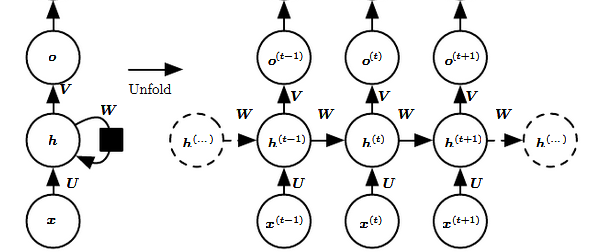
\includegraphics[width=\textwidth]{rnn.png}
	\caption{Architecture of a Recurrent Neural Network (RNN)}
	\label{fig:rnn}
\end{figure}


The left side of the diagram in \ref{fig:rnn} shows a notation of an RNN and on the right side an RNN being unrolled (or unfolded) into a full network. By unrolling we mean that we write out the network for the complete sequence. For example, if the sequence we care about is a sentence of 3 words, the network would be unrolled into a 3-layer neural network, one layer for each word.

\begin{itemize}
	\item Input: $x(t)$ is taken as the input to the network at time step $t$. For example, $x1$, could be a one-hot vector corresponding to a word of a sentence.
	\item Hidden state: $h(t)$ represents a hidden state at time t and acts as "memory" of the network. $h(t)$ is calculated based on the current input and the previous time step's hidden state: $h(t) = f(U * x(t) + W * h(t - 1))$. The function $f$ is taken to be a non-linear transformation such as tanh, ReLU.
	\item Weights: The RNN has input to hidden connections parameterized by a weight matrix $U$, hidden-to-hidden recurrent connections parameterized by a weight matrix $W$, and hidden-to-output connections parameterized by a weight matrix $V$ and all these weights $(U,V,W)$ are shared across time.
	\item Output: $o(t)$ illustrates the output of the network. In the figure \ref{fig:rnn} just put an arrow after $o(t)$ which is also often subjected to non-linearity, especially when the network contains further layers downstream.
\end{itemize}

The gradient computation involves performing a forward propagation pass moving left to right through the graph shown above followed by a backward propagation pass moving right to left through the graph. The runtime is $O(\phi)$ and cannot be reduced by parallelization because the forward propagation graph is inherently sequential; each time step may be computed only after the previous one. States computed in the forward pass must be stored until they are reused during the backward pass, so the memory cost is also $O(\phi)$. The back-propagation algorithm applied to the unrolled graph with $O(\phi)$ cost is called back-propagation through time (BPTT). Because the parameters are shared by all time steps in the network, the gradient at each output depends not only on the calculations of the current time step, but also the previous time steps.
	
	% CONCLUSION
	\chapter{Conclusion}
	The correct behavior of a neural network during the training phase is given by the loss. In a given training step, if the loss is less than or equal to the loss of the previous step then the neural network is working correctly.

The implementation produced was tested with a small dataset and on small neural networks, in order to keep track of the variation of the weights during the training phase. With the passage of the benches and the epochs during the training phase, the loss of the neural networks is lowered or remain constant consequently the training works. In addition, in the most cases, 100\% accuracy is achieved on the training data. In particular, the best results are produced by the RNN.

Further details of testing, profiling and examples will be reported here.
	
\end{document}

